\section{Relationships of organisms with one another and with the environment}
\subsection{Energy flow}
Sun is the principal source of energy input to most biological systems. 

The energy from the sun
is captured into glucose by photosynthesis, that energy is then passed onto other organisms and so
every animal on earth is dependent on photosynthesis.

\begin{center}
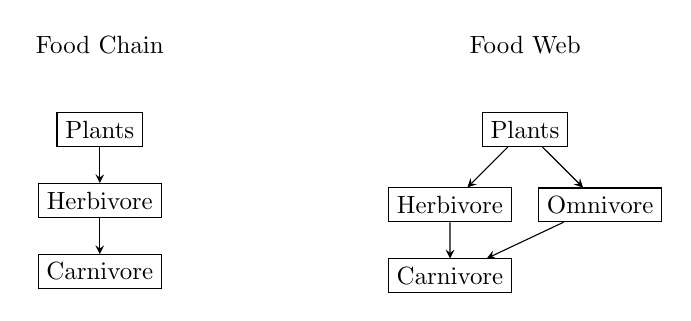
\begin{tikzpicture}[scale=1.2, every node/.style={scale=0.9}, ->,>=stealth]

% Food Chain
\node[rectangle, draw, align=center] (plant) {Plants};
\node[rectangle, draw, below of=plant, node distance=1cm, align=center] (herbivore) {Herbivore};
\node[rectangle, draw, below of=herbivore, node distance=1cm, align=center] (carnivore1) {Carnivore};

\draw[->] (plant) -- (herbivore);
\draw[->] (herbivore) -- (carnivore1);

% Label for Food Chain
\node[above of=plant, node distance=1.2cm] {Food Chain};

% Food Web
\node[rectangle, draw, right of=plant, node distance=6cm, align=center] (plant2) {Plants};
\node[rectangle, draw, below left of=plant2, node distance=1.5cm, align=center] (herbivore2) {Herbivore};
\node[rectangle, draw, below right of=plant2, node distance=1.5cm, align=center] (omnivore) {Omnivore};
\node[rectangle, draw, below of=herbivore2, node distance=1cm, align=center] (carnivore2) {Carnivore};

\draw[->] (plant2) -- (herbivore2);
\draw[->] (plant2) -- (omnivore);
\draw[->] (herbivore2) -- (carnivore2);
\draw[->] (omnivore) -- (carnivore2);

% Label for Food Web
\node[above of=plant2, node distance=1.2cm] {Food Web};

\end{tikzpicture}
\end{center}
Using the two diagramatic structures above, energy flow from one organism to another can be 
represented. A food chain is a diagram showing the flow of energy from one organism to another.
 food web shows that but in multiple interconnected food chains. Both diagrams begin at producers.
Each stage in a food wave or food chain is called a trophic level.

Producers are organisms that make their own organic nutrients, generally using energy from 
sunlight, through photosynthesis. Consumers are organisms that eat these producers to get their
nutrients. 

Herbivores are animals that feed on plants, carnivores are animals that feed on animals.

A decomposer is an organism that gets its energy from dead or waste organic material.

The transfer of energy from one trophic level to another is inefficient for the following reasons:
\begin{itemize}
	\item The organism being eaten has itself respired some of the energy.
	\item Not all of the organism is eaten
	\item Not all of the eaten part of the organism is digested
\end{itemize}

Those that eat consumers are called primary consumers, they are also herbivores. Those that eat
primary consumers are secondary and so on tertiary and quaternary. There are rarely more than five
trophic levels.

In terms of just energy, it is more efficient for humans to eat crops than to eat animals raised on
crops, as energy is lost in two stages when we eat animals, that during photosynthesis from the sun
and that during eating by the animals. Crops provide energy directly captured from the sun and 
hence eating crops is more efficient.

\begin{center}
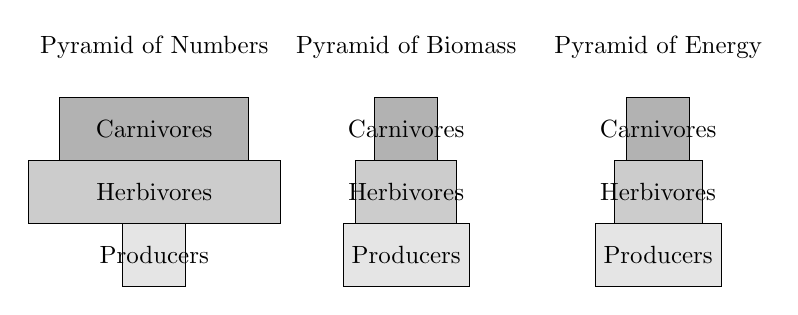
\begin{tikzpicture}[scale=0.8, every node/.style={scale=0.9}, ->,>=stealth]

% Label for Pyramid of Numbers
\node at (0,3.8) {Pyramid of Numbers};

% Pyramid of Numbers (Producers smallest)
\draw[fill=black!10] (-0.5,0) rectangle (0.5,1);  % Producers (smallest)
\draw[fill=black!20] (-2,1) rectangle (2,2);  % Herbivores
\draw[fill=black!30] (-1.5,2) rectangle (1.5,3);  % Carnivores

% Labels inside the boxes for Pyramid of Numbers
\node at (0,0.5) {Producers};
\node at (0,1.5) {Herbivores};
\node at (0,2.5) {Carnivores};

% Label for Pyramid of Biomass
\node at (4,3.8) {Pyramid of Biomass};

% Pyramid of Biomass (Even levels)
\draw[fill=black!10] (3,0) rectangle (5,1);  % Producers
\draw[fill=black!20] (3.2,1) rectangle (4.8,2);  % Herbivores
\draw[fill=black!30] (3.5,2) rectangle (4.5,3);  % Carnivores

% Labels inside the boxes for Pyramid of Biomass
\node at (4,0.5) {Producers};
\node at (4,1.5) {Herbivores};
\node at (4,2.5) {Carnivores};

% Label for Pyramid of Energy
\node at (8,3.8) {Pyramid of Energy};

% Pyramid of Energy (Even levels)
\draw[fill=black!10] (7,0) rectangle (9,1);  % Producers
\draw[fill=black!20] (7.3,1) rectangle (8.7,2);  % Herbivores
\draw[fill=black!30] (7.5,2) rectangle (8.5,3);  % Carnivores

% Labels inside the boxes for Pyramid of Energy
\node at (8,0.5) {Producers};
\node at (8,1.5) {Herbivores};
\node at (8,2.5) {Carnivores};

\end{tikzpicture}
\end{center}
Above are diagrams for the pyramids of numbers, biomass and energy. The pyramid of numbers is
uneven because there may be one huge producer, such as a tree upon which many herbivores depend.

The pyramids of biomass represent the mass of each trophic level and are hence evenly shaped 
because no matter the number of the organisms, the mass will be directly proportional to the
energy at that trophic level.

The pyramid of energy represents the energy at each trophic level.

\subsection{Nutrient cycles}

\textbf{The carbon cycle.} 
The carbon cycle consists of the processes of photosynthesis, respiration, feeding, decomposition,
formation of fossil fuels and combustion.

In photosynthesis, carbon dioxide is absorbed to form glucose using energy from sunlight converted
to chemical energy by chlorophyll. The process occurs in the chloroplasts of plants:

\begin{center}
	\ce{6CO2 + 6H2O -> C6H12O2 + 6O2}
\end{center}
Carbon dioxide in this process is gained from the atmosphere, of which 0.04\% is carbon dioxide. 

In respiration, organisms will use the glucose produced through photosynthesis to release energy,
carbon dioxide and water:

\begin{center}
	\ce{C6H12O6 + 6O2 -> 6CO2 + 6H2O }
\end{center}

The glucose is gained by animals when they feed on plants, or feed on other animals that have fed
on plants. When animals die, decomposers feed on them, also respiring and releasing carbon dioxide.
Those parts of the animals that escape feeding by decomposers, become sedimented, are compressed
underground and form fossil fuels, which can be combusted, again releasing carbon, to be absorbed
by plants during photosynthesis again.

\textbf{The nitrogen cycle.} Living things need nitrogen to make proteins and DNA. In the 
atmosphere, nitrogen is in the molecular form \ce{N2}, which is a triply bonded molecule: 
\chemfig{N~N}. These molecules are very inert in that they do not easily react to many substances.
This unreactive nitrogen must be converted to reactive forms, which are ammonia (\ce{NH3}) and
nitrates (\ce{NO3-}). This process is called nitrogen fixation.

Nitrogen fixing occurs during lightning, where the lightning makes the nitrogen gas combine with
oxygen in the air, forming nitrogen oxides, which dissolve in rain and wash into the soil, where
they form nitrates. Nitrogen and hydrogen react in an industrial chemical process, forming ammonia,
which is used to make ammonium compounds and nitrates, which can be used to make fertilisers. 
There are bacteria that live in the soil or root nodules (small swellings) on plants such as peas,
beans or clover, called nitrogen-fixing bacteria. The use nitrogen from the air spaces in the
soil and combine it with other substances to make ammonium ions and other compounds. Plants can
use this fixed nitrogen to make amino acids which can then be used to make their proteins, which
animals digest and get their nitrogen in the form of nitrogen. When an animal or plant dies,
bacteria and fungi decompose the body, turning the amino acids into ammonium ions. Bacteria then
convert this ammonium to nitrates, through a process called nitrification. They are hence named
nitrifying bacteria. Another group of bacteria convert nitrates and ammonia in the soil to nitrogen
gas, through a process called denitrification, and they are hence named denitrifying bacteria.

\subsection{Ecosystems and biodiversity}

A population is a group of organisms of one species, living in the same area, at the same time.
A community is all of the populations of different species in an ecosystem. An ecosystem is a unit
containing the community of organisms and their environment, interacting together.

Biodiversity is the number of different species that live in an area.

The factors that affect the rate of population growth for a population of an organism boil down to
the following:
\begin{itemize}
	\item Food supply: The more the food available for a population, the faster they it will grow.
	\item Competition: The more the competition for resources amongst populations, the slower they
		will grow.
	\item Predation: The more the predation for a certain population, the slower they will grow.
	\item Disease: The more affected a population is by disease, the slower its growth.
\end{itemize}
The opposite also apply for all the above factors.

For humans, all these factors are favourable, causing an exponential increase in the human 
population. All these people result in an increased demand for global resources.

\subsection{Effects of humans on ecosystems}

\textbf{Deforestation.} 
Deforestation results in loss of biodiversity, habitats of animals will be lost, who may become
extinct for lack of places to habitable regions. Trees hold in soil with their roots, in their
absence, during excessive rain, soil may wash into water bodies, being lost. Trees absorb water
after rainfall, in their absence the water remains and causes flooding. Lack of trees means that
carbon dioxide will not be absorbed as much during photosynthesis, resulting in a higher carbon
dioxide concentration in the atmosphere.
